\documentclass[11pt, letter,twocolumn]{article}
\usepackage[margin=0.75in,  ]{geometry} % columnsep=0.2in
\usepackage{amsmath,amsthm,amsfonts,amssymb,amscd}
\usepackage{mathrsfs}
\usepackage{graphicx}
\usepackage{float}
\usepackage{outlines,enumitem }
\usepackage{hyperref}
\usepackage{esvect}
\usepackage{placeins} % FloatBarrier force new section after an image
\usepackage{fancyhdr}
\usepackage{svg}
% -- upper right corner main info
\usepackage{outlines}
\usepackage{abstract}
 
%\setlength{\jot}{15pt} % vertical space between math
%\setlength\parindent{0pt} % no indent
%\setcounter{secnumdepth}{0} % no section counting
\usepackage[
backend=biber,
style=authoryear,
sorting=nty
]{biblatex}
 \addbibresource{ref.bib} 
 % ---------------
 % Macro 
 
 % -- add parentheses in fraction espression if there is a superscript. 
 \makeatletter
 \let\old@frac=\frac
 \def\frac#1#2{%
 	\@ifnextchar^
 	{\left(\old@frac{#1}{#2}\right)}
 	{\old@frac{#1}{#2}}%
 }
 
 \let\old@dfrac=\dfrac
 \def\dfrac#1#2{%
 	\@ifnextchar^
 	{\left(\old@dfrac{#1}{#2}\right)}
 	{\old@dfrac{#1}{#2}}%
 }
 
 \makeatother
% inner product
 \newcommand\inner[2]{\langle #1, #2 \rangle}

 % -----------------
 
%  https://tex.stackexchange.com/questions/279100/typeset-the-shrug-%C2%AF-%E3%83%84-%C2%AF-emoji
 \usepackage{graphicx,rotate}
 \newcommand{\teamname}{
\rule[1.3ex]{.25em}{1pt}\kern-.1em%
\reflectbox{\small\ttfamily/}%
\kern-.1em\rule[-.2ex]{.4em}{1pt}%
\makebox{{\raisebox{.15em}{{\large\textcircled{
					\ttfamily\kern-.35em%
					\rotatebox[origin=t]{-120}{\bfseries\scriptsize`\kern-.3ex`}%
					\kern-.15em\rotatebox{-45}{\bfseries\scriptsize)}}}}%
		\rule[-.2ex]{.4em}{1pt}\kern-.1em{\small\ttfamily/}%
		\kern-.1em\rule[1.3ex]{.25em}{1pt}}} 

}
 
\begin{document}

\title{Report for Econometric Competition on Predicting 2019 Individual Income}
\author{Team:  \teamname \\ Member: Hengyu Kuang}
\maketitle

\begin{abstract}
We build an ensemble model from LightGBM and Transformer based neural net to predict 2019 individual annual pre-tax wage and salary. The error analysis suggests college and graduate students have the highest error, and ages in both tails have unbalanced errors. We find    mean square error weighted by education   gives lower overall error. We follow the competition rules and add magics in the final prediction. Codes are available in the github page. 
\end{abstract}



\section{Preliminary Data Analysis }
Data is a subset of 2019 American Community Survey obtained from IPUMS (\cite{ruggles_ipums_2021}). The goal is to predict individual pre-tax wage and salary  using 12 variables. The evaluation metric is mean square error of log income. 

The dependent variable, incwage, is non-negative integer and ranges within [0, 999999].  999999 is encoded as  N/A, and  999998 means missing. Neither values are in the samples. Dependent variables are sex, age, martial status (marst), race, birthplace (bpl), language, educational attainment (educ), occupation (occ), weeks worked last year (wkswork1), hours worked per week (uhrswork), and veteran status (vetstat). All independent variables are pre-encoded as integers. 
% \begin{table}[h!]
    \centering
    \begin{tabular}{|l|l|l|l|}
    \hline
    Variable & Variable Label              & UniqueN & Note                           \\ \hline
    incwage  & wage and salary income      & 946     & 999999 = N/A; 999998 = Missing \\ \hline
    sex      & sex                         & 2       &                                \\ \hline
    age      & age                       & 81      &                                \\ \hline
    marst    & marital status              & 6       &                                \\ \hline
    race     & race                        & 9       &                                \\ \hline
    bpl      & birthplace                  & 123     &                                \\ \hline
    language & language spoken             & 63      &                                \\ \hline
    educ     & educational attainment      & 11      & 00 = N/A or No School          \\ \hline
    degfield & field of degree             & 38      & 00 = N/A                       \\ \hline
    occ      & occupation                  & 529     & 00 = N/A                       \\ \hline
    wkswork1 & weeks worked last year      & 52      & 00 = N/A                       \\ \hline
    uhrswork & usual hours worked per week & 99      & 00 = N/A; 99 (top code);       \\ \hline
    vetstat  & veteran status              & 3       & 0 = N/A                        \\ \hline
    \end{tabular}
    \end{table}

The training data has 318,074 rows, and the test data has 1,272,344 rows. The training data has 1,404 (0.44\%) duplicated rows. 1,274 (90.74\%) of them  have 2 duplicates, and 119 (8.47\%) have 3 duplicates. The test data has 86,804 (6.82\%) duplicated rows. We expect the independent variables fail to provide enough information to identify the income variable. 

Numeric variables are age, hours worked last year (whrswork) , weeks worked last year (wkswork1). They can also be treated as categorical variables as value ranges are fixed integers.

Categorical independent variables are the remaining 9 variables with various levels. Specifically, Birthplace (bpl) has 123 levels, occupation (occ) has 529, and language spoken has 63. 

The distribution on income is right-skewed with mean 54,278, median 38,000, and std 68086.31. The top 10\% quantile is 110,000, and bottom 10\% is 5,000. Figure \ref{fig:distributionlogincome} shows the distribution on log of income. It's approximately normal with mean  10.29 and std 1.299.    

\begin{figure}[ht]
	\centering
		\caption{}
	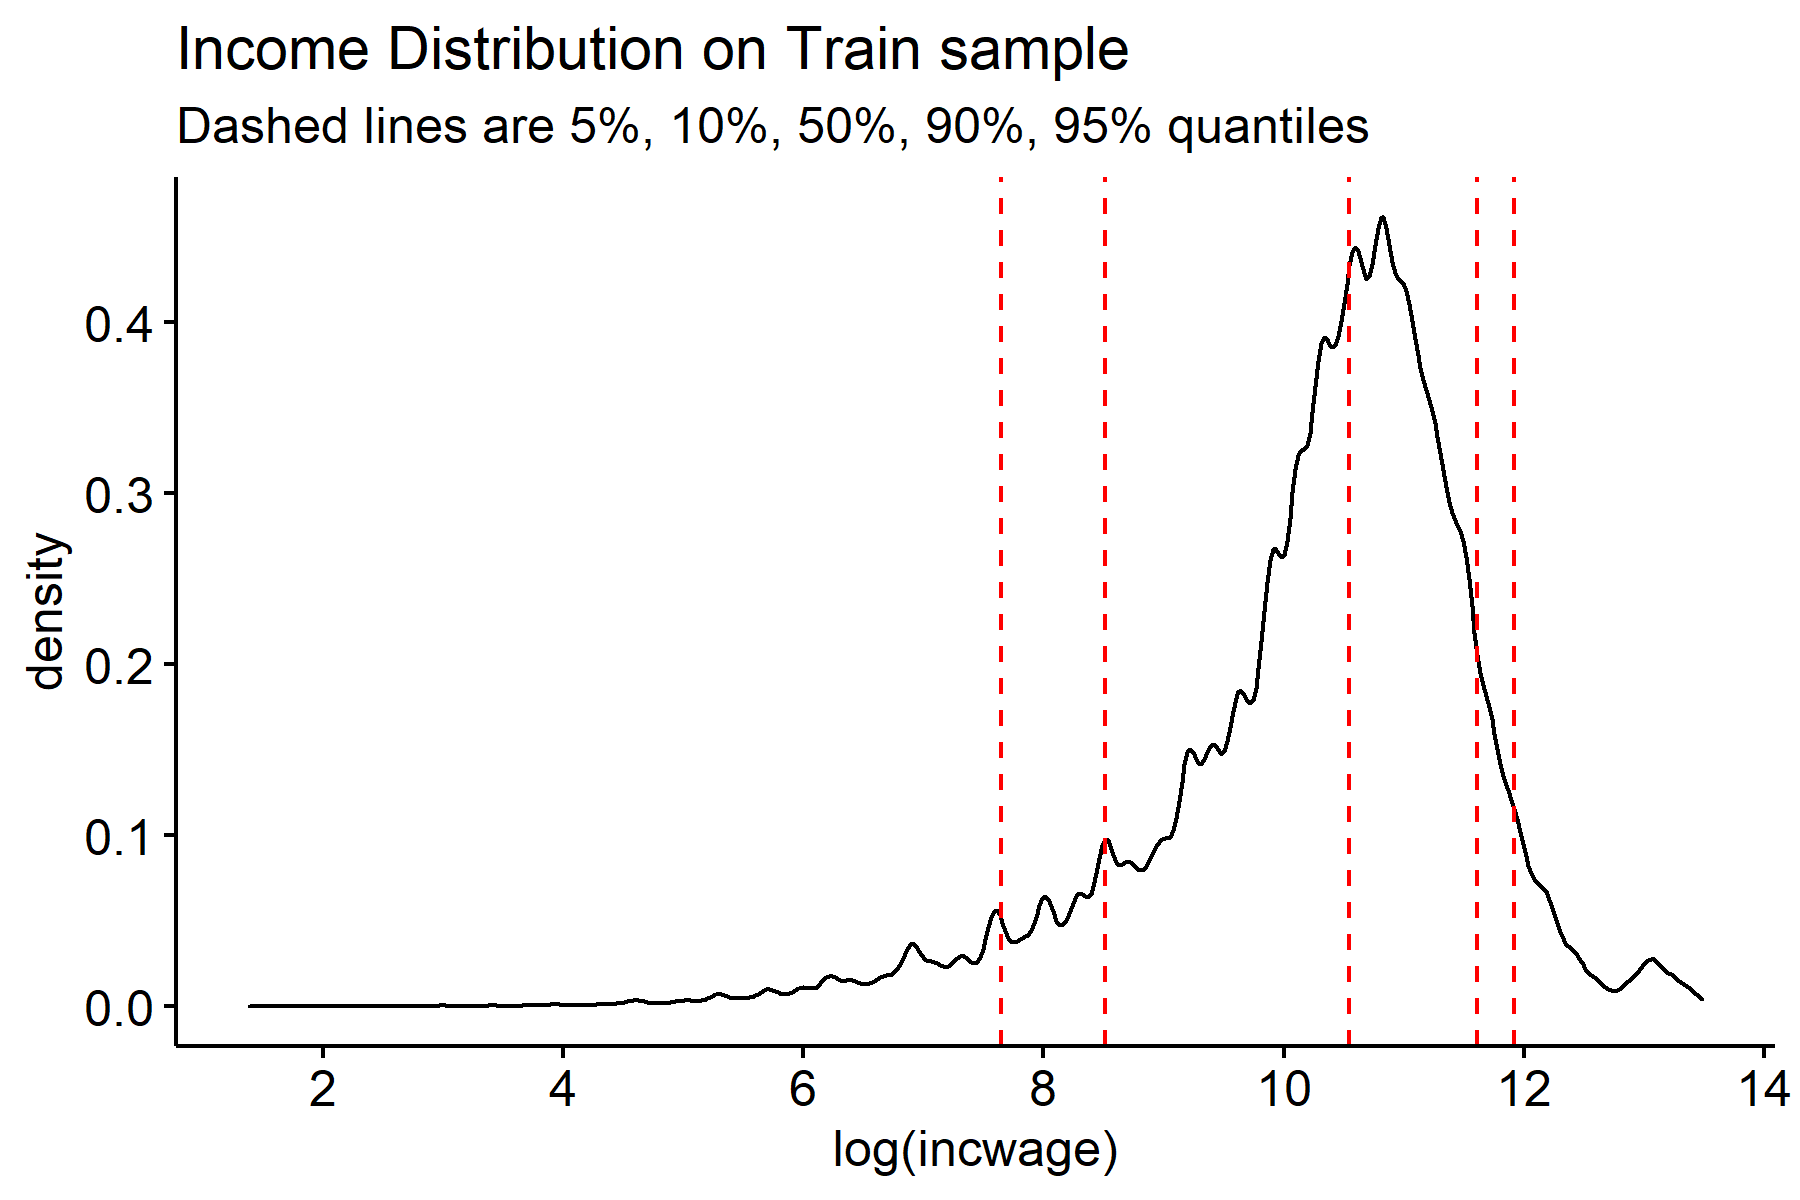
\includegraphics[width=0.9\linewidth]{imgs/distribution_log_income}
		\label{fig:distributionlogincome}
\end{figure}

All independent variables in the train and test sets have approximately the same distributions. Both non-parametric Kruskal-Wallis tests and ANOVA  fail to reject the null hypothesis that the independent variables in the two datasets have different means.

In the training sample, average high income groups are EU member counties (bpl in 400 range) and minority language speakers. The White (race=1)  people has the most observations, but their average income ranks the 4th. Asian populations are in the highest average income group. STEAM majors also have the highest average income.  

We highlight income against education and age. Additional plots on comparing variable distributions are in the appendix.

Figure \ref{fig:incwageeduc} shows people with higher educations have much higher income. More than 5 years of college (educ = 11) account 14.29\% of the training sample, and their average income is more than 100,000. College students (educ=10,8,7) ranked second, and are followed by high school graduates (educ=6).
 

\begin{figure}[ht]
	\centering
		\caption{}
	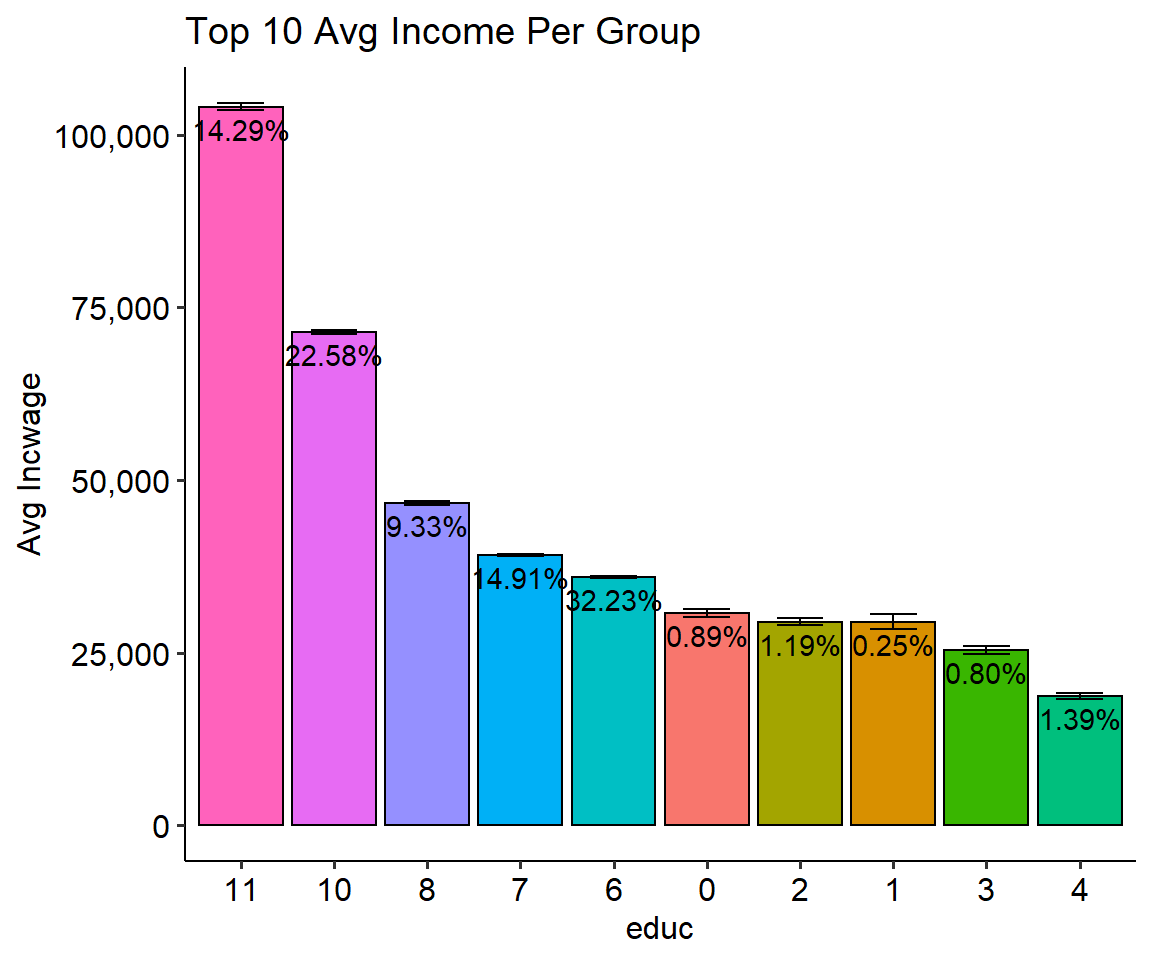
\includegraphics[width=0.9\linewidth]{imgs/incwage_educ}
		\label{fig:incwageeduc}
\end{figure}

Figure \ref{fig:incwageage} shows young people with age less than 25 tend to have much lower income compared to middle age. However, the senior group has larger variance. We expect young and highly educated people have less income in their early careers.

\begin{figure}[ht]
	\centering
	\caption{ }
	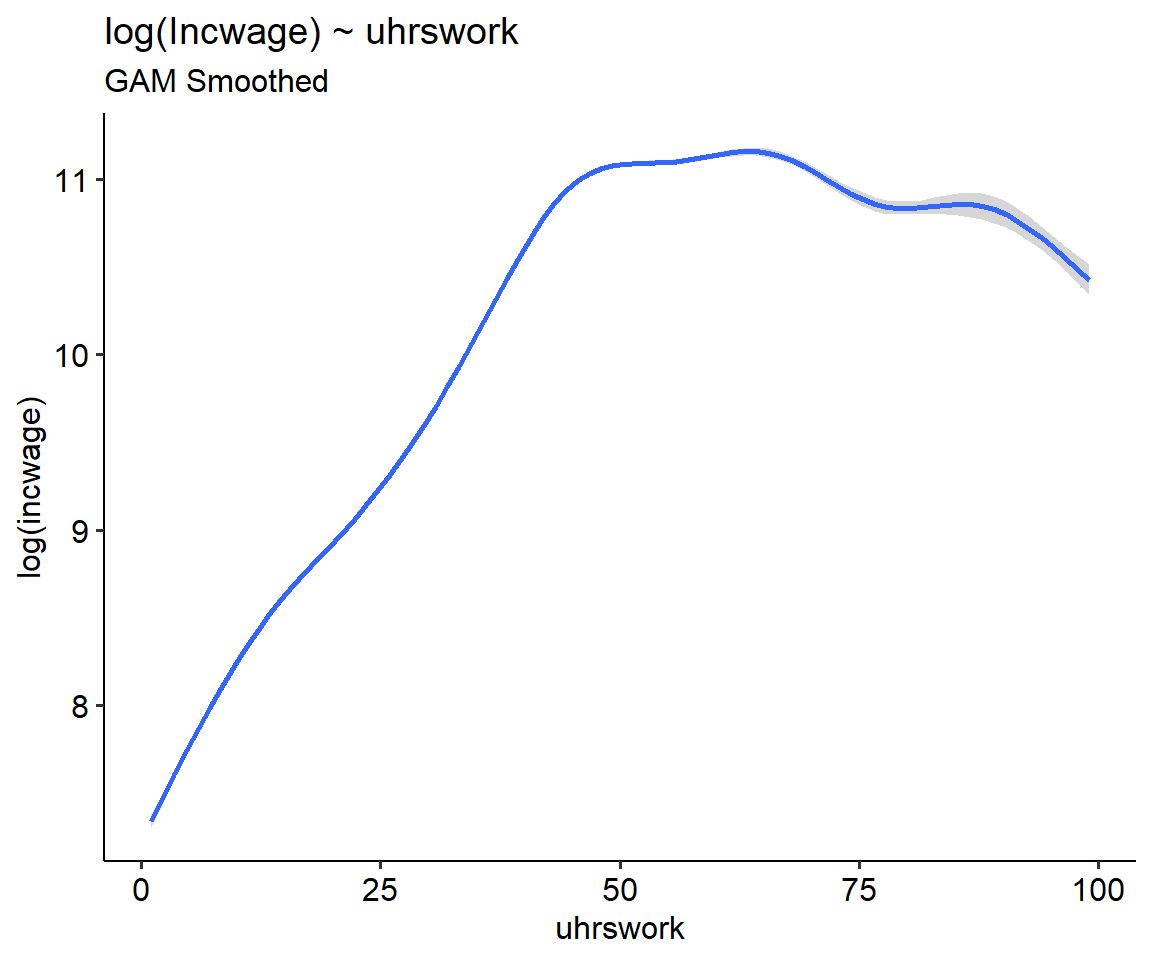
\includegraphics[width=0.9\linewidth]{imgs/incwage_age}
		\label{fig:incwageage}
\end{figure}

\section{Models}
The categorical variables have large amount of levels, and there are duplicate rows. Instead of using linear models, we use    gradient boosting trees   and   Transformer based neural networks to build the final ensemble model. 

\subsection{Boosting Trees  }
We compare Light Gradient Boosting Machine (LightGBM) \parencite{ke2017lightgbm},   Categorical Boosting (CatBoost) \parencite{dorogush2018catboost}, and Extreme Gradient Boosting (XGBoost) \parencite{XGBoost2016}. LightGBM consistently outperforms other tree models by 4\% to 15\% in subsets of the training data, and in mixed ensemble trees its predictions have much higher weights, so we choose LightGBM.

We use the Python package ``AutoGluon'' \parencite{erickson_autogluon-tabular:_2020} implantation and use Bayesian optimization to search hyper-parameters.  

\subsection{Neural Networks}
We compare 3 basic architectures: Residual Multi-layer Perceptions,  Convolutional neural net, and Transformer based nets. Transformer models have the best performance and fastest convergence. 
Figure \ref{fig:transformerarchitecture} shows the architecture of a modified Transformer. It contains column wise embedding layers for each variables, Transformer layers as encoder, and a dense layer for output prediction. 

B denotes the number of observations, $ M_1 $ is number of categorical column, $ M_2 $ is the number of numerical columns, and $ M = M_1 + M_2 $. The embedding layer, a list of linear transformations, maps each independent variable into a D dimensional vector that are then passed into  Transformer layers. The final dense layer includes two linear transformations: one for the dimension M that combines all independent variables into 1, and the other one maps the dimension D into a real number. Dropout layers are placed both in the feed forward layer and multi-head attention layer. 

 \begin{figure}[ht]
 \centering
 \caption{Transformer Architecture}
 \label{fig:transformerarchitecture}\vspace{1em}
 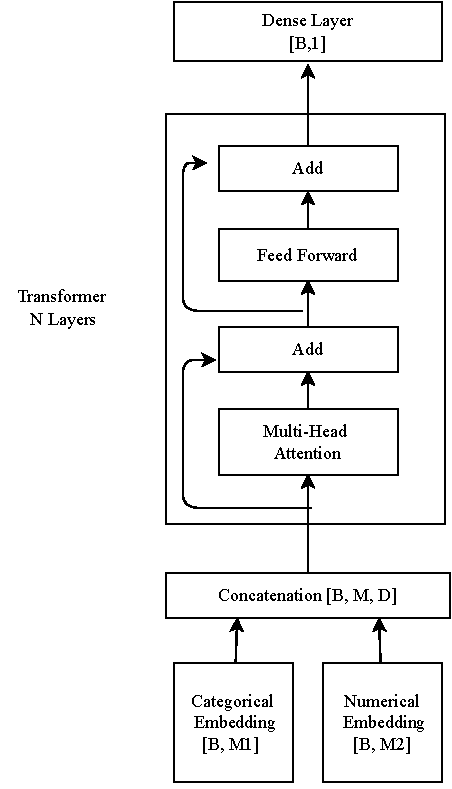
\includegraphics[width=0.8\linewidth]{imgs/transformer_architecture.pdf}
\end{figure}


\textcite{narang2021transformer} shows the vanilla Transformer is good enough and empirically shows Gated Linear Units (GEGLU) and Root Mean Square Norm (RMS Norm) outperform  recent modifications.  \textcite{huang_improving_2020} theoretically show   proper model initialization can bound the variance in optimization update steps and thus eliminate the learning rate warn up and  layer norms.   We follow their initialization scheme and remove all layer norms in the Transformer layer. We also replace non linear activation by GEGLU in the feed forward block. 

Hyper-parameters include number of Transformer Layer N, embedding dimension $ D $,  feed forward hidden dimension, multi-head dimension, batch size,  weight decay, learning rate, and dropout. 

We use Pytorch \parencite{paszke_pytorch:_2019} and Pytorch Lightning \parencite{falcon2019pytorch} to build neural nets.


\section{Experiments}

We start with a small subset of data to test various model settings and narrow down parameter search space. We use  40\% of  data as training set, 10\% as validation set, and 10\% as test set. All models are trained on the same dataset and benchmarked in the same test set. The evaluation metric is  Mean Square Error (MSE) on the log of income.

We find treating numeric variables as categorical yield better results for neural nets but worse for tree models. Tree models use standardized age, hours worked, and weeks worked last year as numeric variables. 
The error analysis suggest we get better performance by  penalizing higher weights for college students and grouping ages separately for below 25 and over 75.   




In the fine-tuning phrase, we split the data into 90\% training and 10\% validation. Models are early stopped by monitoring the validation set.


\subsection{Parameter Search}
In the tree models, we use  ``Autogluon'' default parameter search space for XGBoost and CatBoost as they already control out of sample variance. But we add regulizations  parameters  for the LightGBM. They are ``bagging\_fraction'', ``bagging\_freq'', ``lambda\_l1'', ``lambda\_l2''.  Parameter search is based on Gaussian process Bayesian optimization. Self-ensemble models are reported in table \ref{tab:my-table}.
 \begin{table}[ht]
	\caption{Ensemble Trees in Test Set}
	\label{tab:my-table} 
	\centering \vspace{1em}
	\begin{tabular}{ll}
		\hline
		Model    & MSE    \\
		\hline
		\textbf{LightGBM} & \textbf{0.5156} \\
		XGBoost  & 0.5333 \\
		CatBoost & 0.5325 \\ 
		\hline
	\end{tabular}
\end{table}


In the neural nets, we use Adam for optimization and train models in mixed precision (FP16/FP32), resulting in faster convergence and lower GPU memory consumption. We fix batch size at 2048 as we find larger batches have no impact on test results.  We first search optimal combinations on learning rate (LR), transformer layers (N), feed forward dimension (FF), and embedding (E). Then, we find dropout and weight decay for regularization. 

Models are early stopped when there are no improvement in the validation set for 10 epochs or when gradient explode. All models are then benchmarked in the test set. Selected results are reported in table \ref{tab:architeture}.  
 
\begin{table}[ht]
\caption{Transformers in Test Set}
\label{tab:architeture}
\centering \vspace{1em}
\begin{tabular}{llllll}
\hline
LR & E    & FF &  N & Parameters       & MSE   \\
\hline
8e-4          & 128          & 512          & 4                  & 1.442 M          & NA              \\
6e-4          & 128          & 512          & 4                  & 1.442 M          & 0.5745          \\
4e-4          & 128          & 512          & 4                  & 1.442 M          & 0.5842          \\
6e-4          & 64           & 256          & 4                  & 0.393 M          & 0.6269          \\
6e-4          & 256          & 1024         & 4                  & 5.506 M          & 0.5578          \\
\textbf{6e-4} & \textbf{128} & \textbf{512} & \textbf{6}         & \textbf{2.100 M} & \textbf{0.5562} \\
6e-4          & 128          & 512          & 6                  & 2.100 M          & 0.5591          \\
4e-4          & 128          & 512          & 6                  & 2.100 M          & 0.5641          \\
6e-4          & 128          & 256          & 6                  & 1.507 M          & 0.5865       \\ 
\hline
\end{tabular}
\end{table}

We find learning rate larger than 2e-3 guarantees gradient explosion, and 8e-4  is not stable.  Deeper models seem to perform better than wider models, but they require longer training time and heavier regularizations. Wider models also bottleneck training in the multi-head attention blocks. We try Sparsemax to replace softmax in the attention block, and we find it benefits larger models as it creates extra regularization by zeroing out less useful features. However, the training time is much longer.    

We decide to use 128 embedding size, 512 feed forward dimension, 6 Transformer layers, and 6e-4 learning rate. We  find 5e-5 weight decay and 0.4 dropout have the best performance. 

We also try to replace the dense layer by residual blocks, but models quickly overfit the  data. We also try an image model by converting the embedding layer into an image-like structure, which is a 4 dimension tensor with batch size, number of variables, img width and img height, and then pass into the Efficient Net V2 \parencite{tan_efficientnetv2:_2021}. But performances are much worse than Transformers. 



\subsection{Error Analysis}
Tree models report age, hours worked per week (uhrswork), and education are import features. We find age and education gives the highest unbalance prediction error. 

The histogram in figure \ref{fig:erroranalysisoneduc} shows the majority of large errors are from high school and college graduates. Figure \ref{fig:erroranalysisonage} shows the prediction errors larger than 10,000. Young people and seniors have the largest error prediction, and graduates with more than 5 years of college study have the highest unbalanced distribution. We expect the recent graduates have lower income in their early careers. 



\begin{figure}[ht]
	\centering
	\caption{}
	\label{fig:erroranalysisoneduc}
	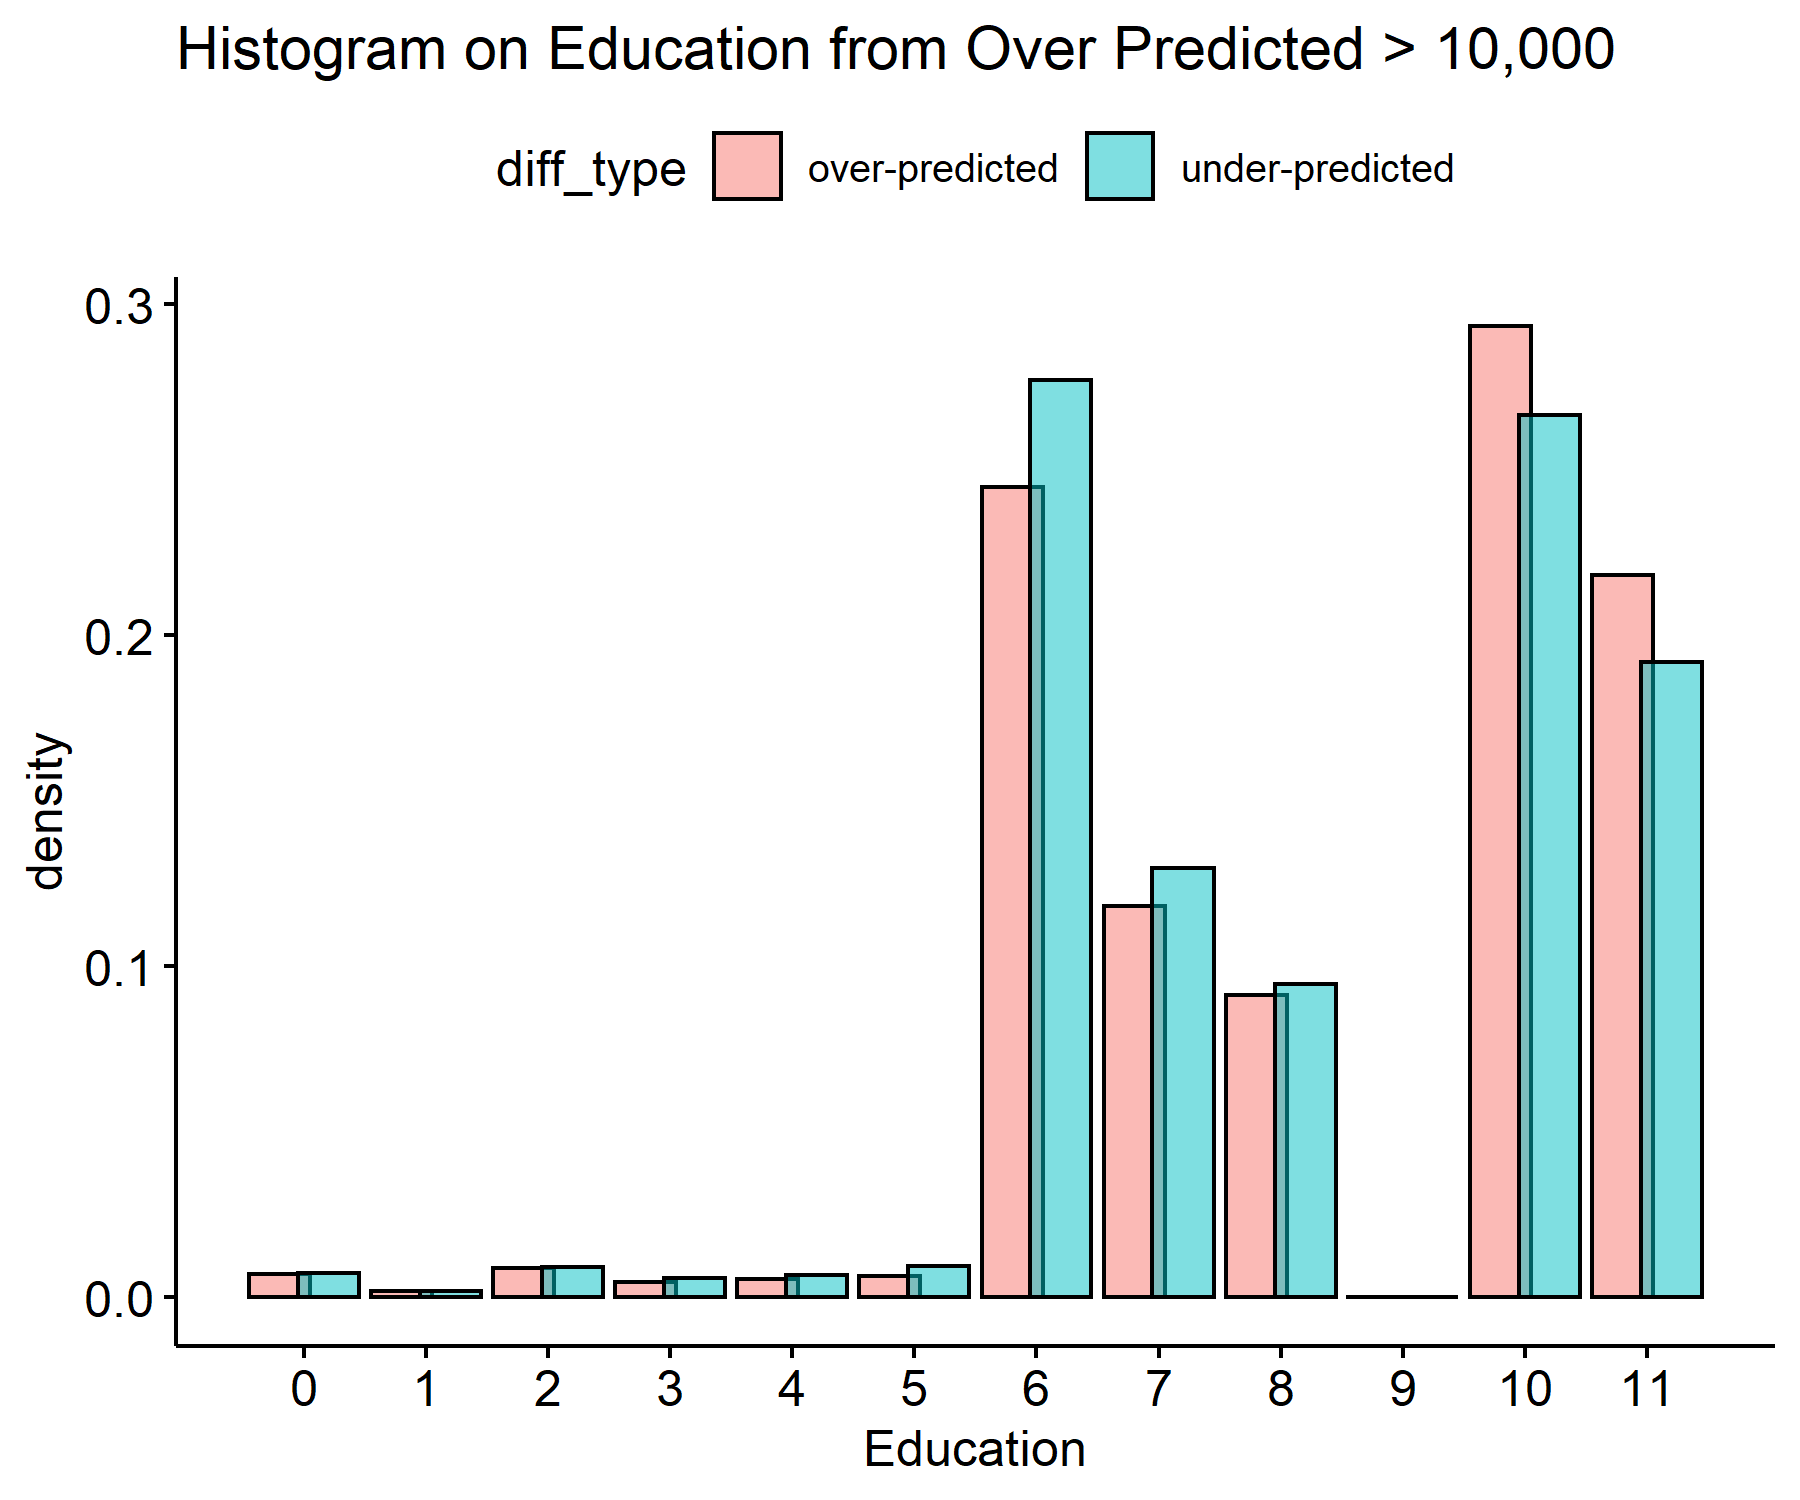
\includegraphics[width=0.9\linewidth]{imgs/error_analysis_on_educ}
\end{figure}


\begin{figure}[ht]
	\centering
	\caption{}
	\label{fig:erroranalysisonage}
	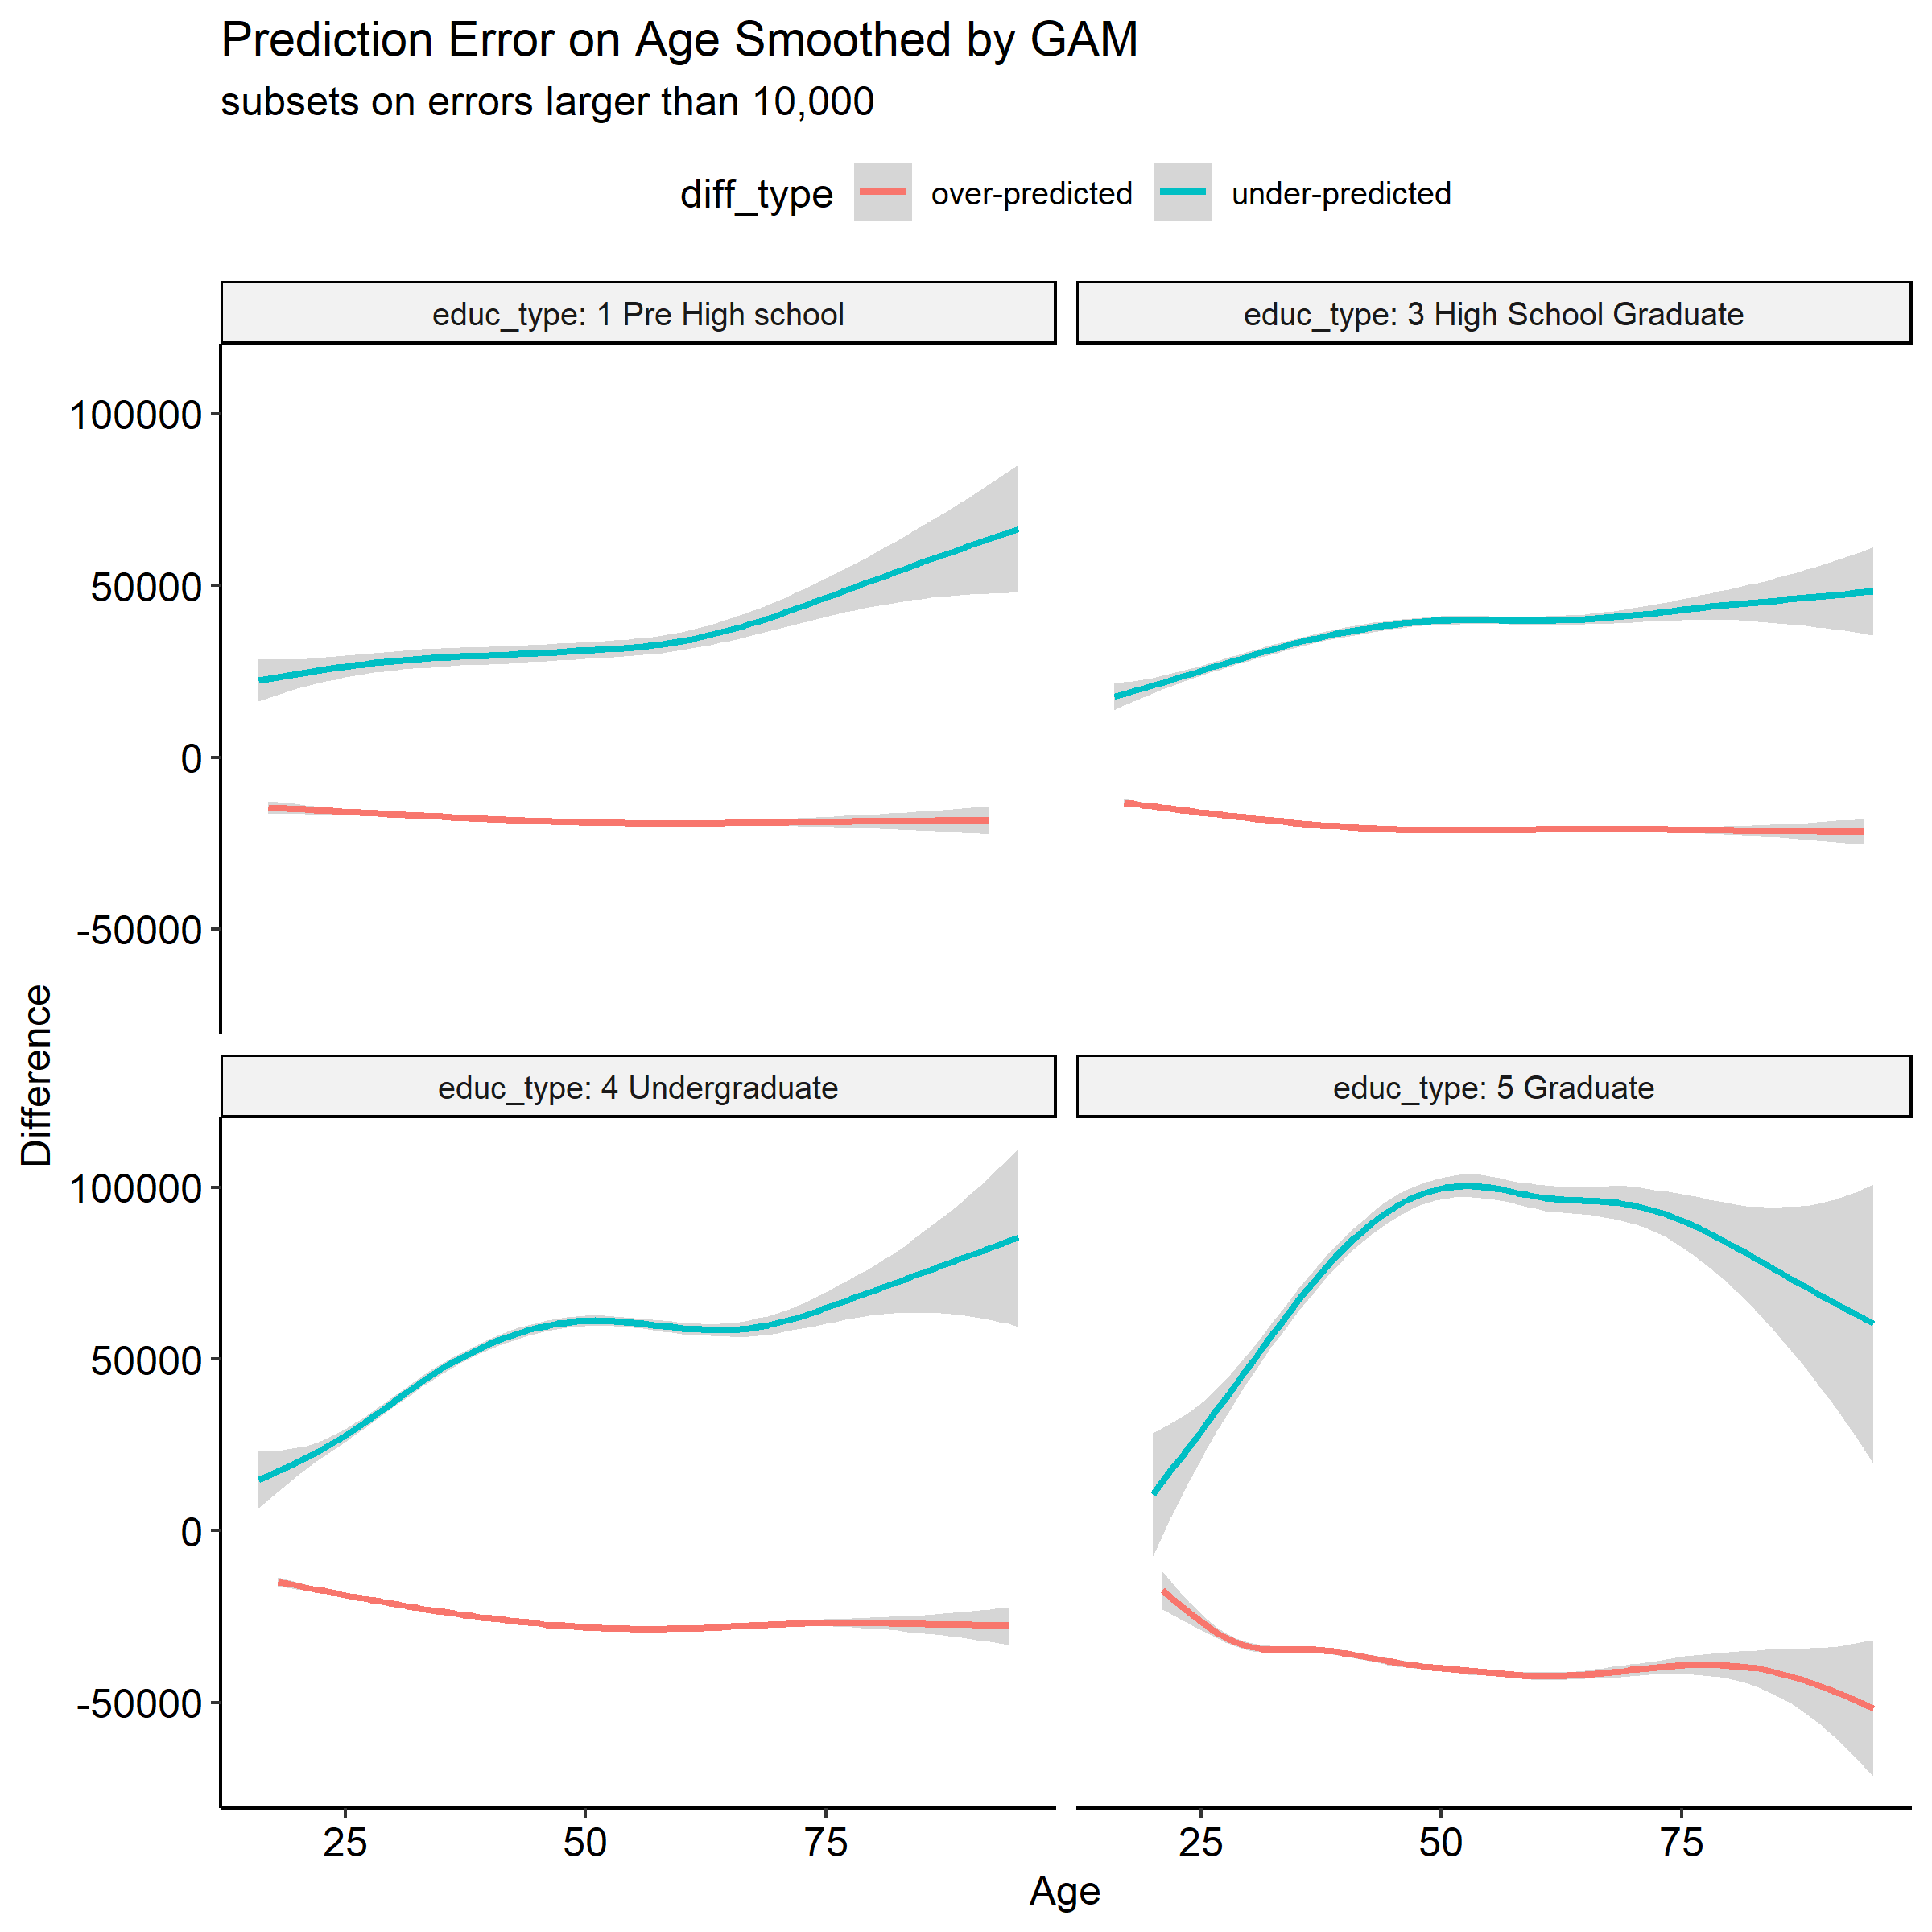
\includegraphics[width=0.9\linewidth]{imgs/error_analysis_on_age}
\end{figure}
We re-run both models with different feature settings. In tree models, pre college observations have weight of 1, colleges with 1-4 years of study have weight of 2, and graduates have weight of 3. We compare auto weight search, manual settings, and equal weights. In neural nets, we add the same weights in the loss function. We also group ages below or equal to 25 as 1 group and ages above or equal to 75 as another group.  
Results are listed in table \ref{tab:my-table_penalty}. The feature engineering is effective.

 \begin{table}[ht]
	\caption{Feature Engineering in Test Set}
	\label{tab:my-table_penalty} 
	\centering \vspace{1em}
	\begin{tabular}{lll}
		\hline
		Model   & Penalty \&  Grouping & MSE    \\
		\hline
		LightGBM & False  & 0.5156 \\
		\textbf{LightGBM}  & \textbf{True}  & \textbf{0.5010}\\
		Transformer  & False & 0.5562\\
		\textbf{Transformer}  & \textbf{True} & \textbf{0.5312} \\
		\hline
	\end{tabular}
\end{table}
\subsection{Fine Tuning}

We train the two models on the full sample. Hyper-parameter search space for LightGBM is narrowed according to previous experiments and increase search iterations. Neural nets learning rates are adjusted lower by multiplying 0.8 when there are no improvement for 5 epoch. Model is early stopped when there are no improvements for 20 epochs in the validation set.   To build a mixed ensemble mode, we try a simple weighted average on the two. The optimal weight for LightGBM is 0.999, meaning Transformer has no usage. We also use the predictions as  features to train  ensemble trees in LightGBM that gives slightly better performance. 

 
Table \ref{tab:my-table_penalty_full_sample}   shows the MSE for the whole training set. The final prediction on the test set is  round$(\exp(\log(incwage)))$ as it has around 3e-8 less error than rounding down or up. We find adding magics yields much better performance, so we use it for the final submission.
 
\begin{table}[ht]
 	\caption{Full Training Sample}
 	\label{tab:my-table_penalty_full_sample} 
 	\centering \vspace{1em}
 	\begin{tabular}{lll}
 		\hline
 		Model   &    MSE    \\
 		\hline
 		LightGBM    & 0.3901 \\
 		Transformer     & 0.4265\\
 	    Mixed Ensemble (Weighted)    & 0.3990\\
 		\textbf{Mixed Ensemble (Trees)  }   & \textbf{0.3873}\\
 		Magics &  ?? \\
 		\hline
 	\end{tabular}
 \end{table}




\FloatBarrier
\printbibliography 
\newpage
\appendix
\section{Additional Plots on Preliminary Data Analysis}
There are almost no difference in the train and test samples. Neither ANOVA nor Kruskal-Wallis test reject the null hypothesis that the two dataset have different distribution in any independent variables.

 If we only look at single variable against income, we have the following observations:
\begin{outline}
	\1 male(sex=1) has slightly higher income than female (sex=2);
	\1 married (marst=1) has the most observation and highest income; but single (marst=6) has the second most observation and lowest income;
	\1 white (race=1) has the most observation but income ranks at 4th; Chinese, Japanese, other asian (race=4,5,6) have less observations but highest income; 
	\1 EU member counties (bpl in 400 range) have the highest income
	\1 minority language speakers have the highest average income
	\1 5 years + college (educ=5) and 4 years + (educ=4) are the top earners.
	\1 Engineering, Transportation Sciences and Technologies, Biology and Life Sciences (degfield = 24, 59, 36) have the highest avg income.
\end{outline}

If we use embedding for each category variables, degfield shall get special attention, followed by educ as they seem to have high predictive power. language and bpl may need to consider sparse setting as the majority speakers are English speakers born within the U.S., but they have diverse income.

\begin{figure}[ht]
	\centering
	\label{fig:unnamed-chunk-7-1}
	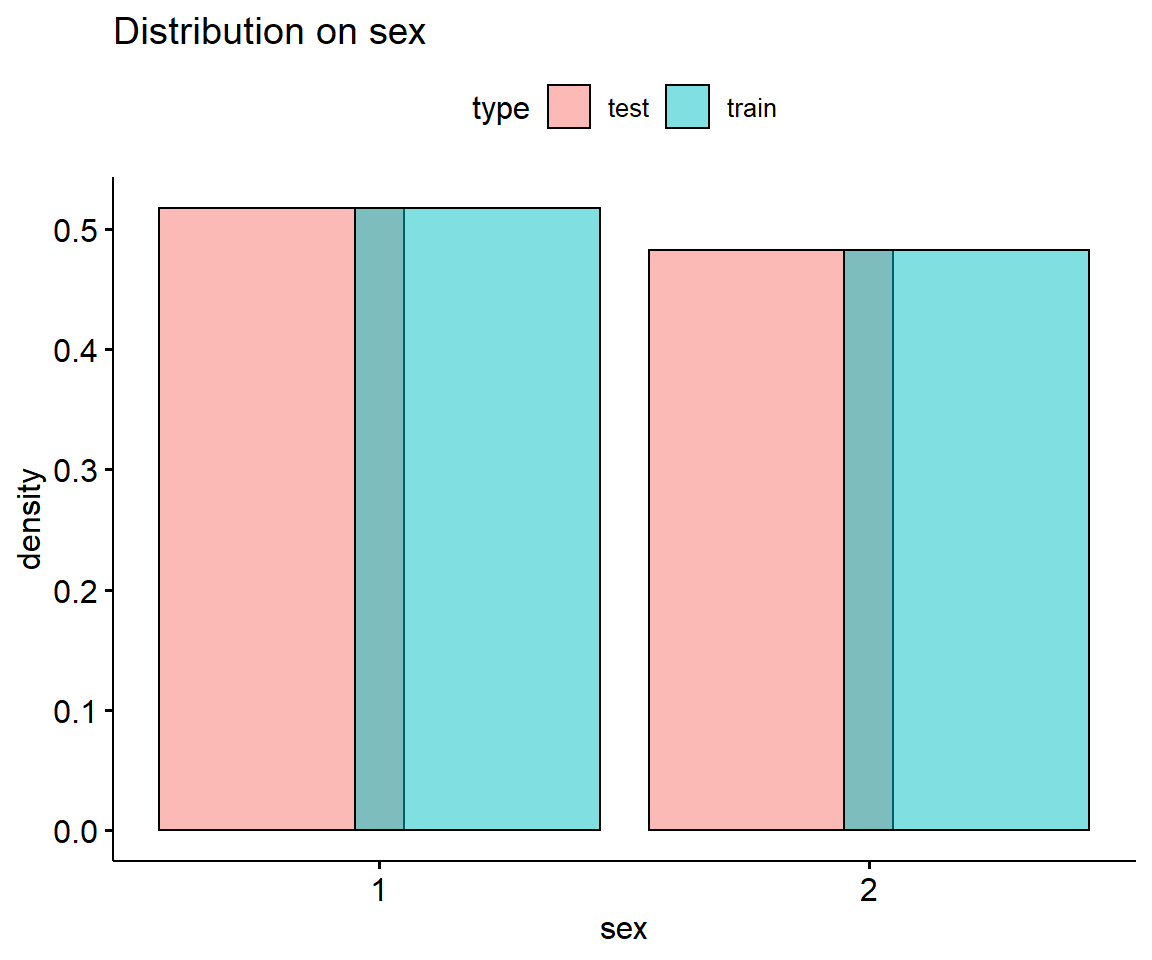
\includegraphics[width=0.9\linewidth]{imgs/preliminary_analysis/unnamed-chunk-7-1}
\end{figure}

\begin{figure}[ht]
	\centering
	\label{fig:unnamed-chunk-7-2}
	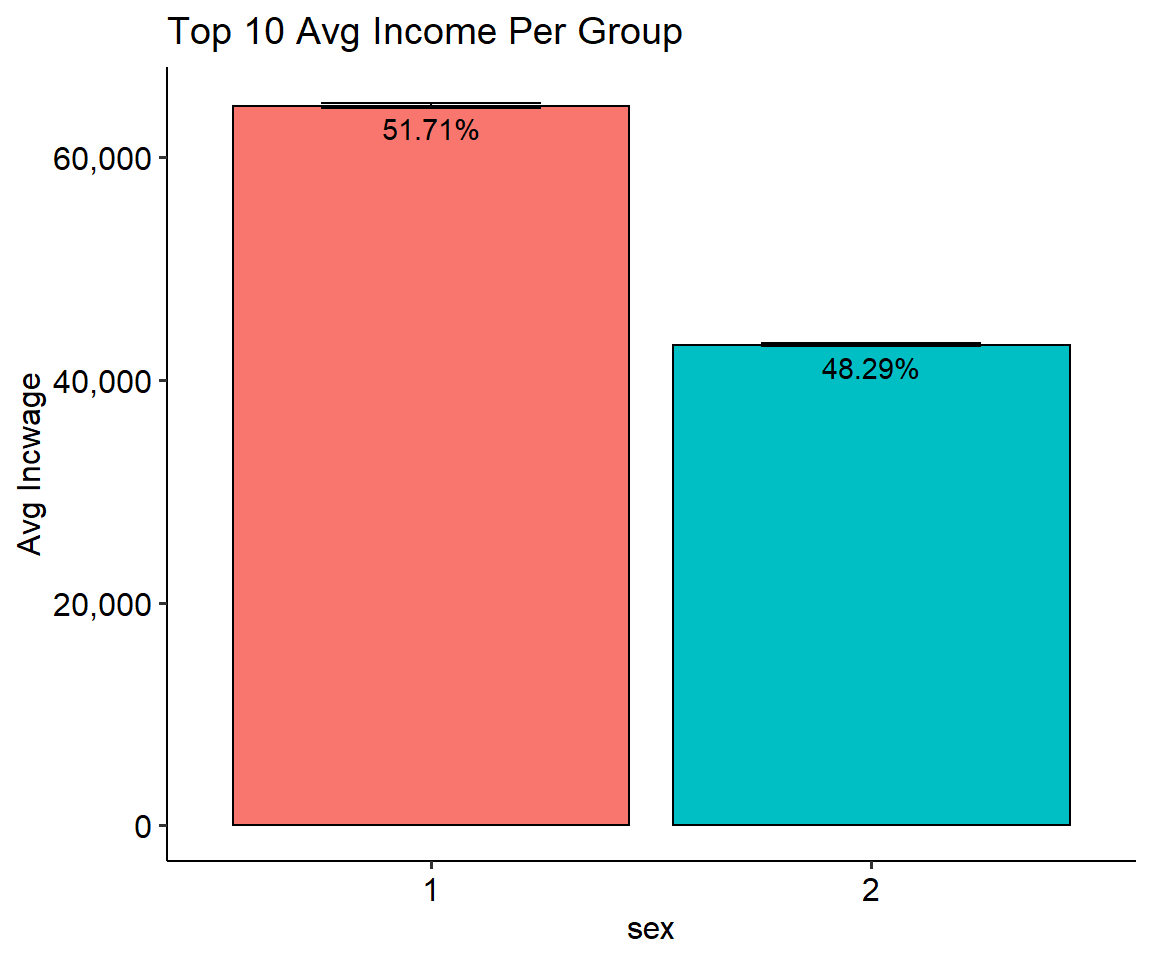
\includegraphics[width=0.9\linewidth]{imgs/preliminary_analysis/unnamed-chunk-7-2}
\end{figure}


\begin{figure}[ht]
	\centering
	\label{fig:unnamed-chunk-7-3}
	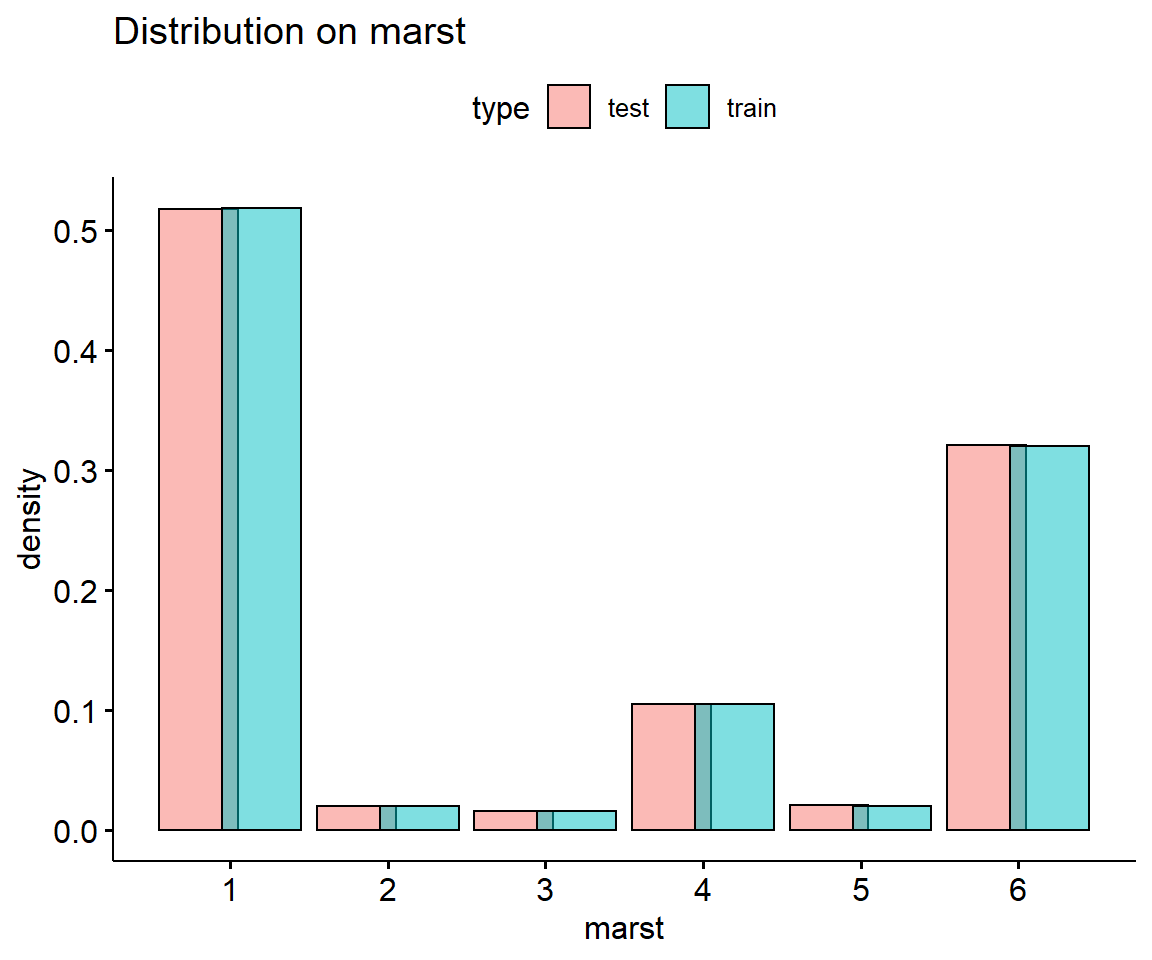
\includegraphics[width=0.9\linewidth]{imgs/preliminary_analysis/unnamed-chunk-7-3}
\end{figure}


\begin{figure}[ht]
	\centering
	\label{fig:unnamed-chunk-7-4}
	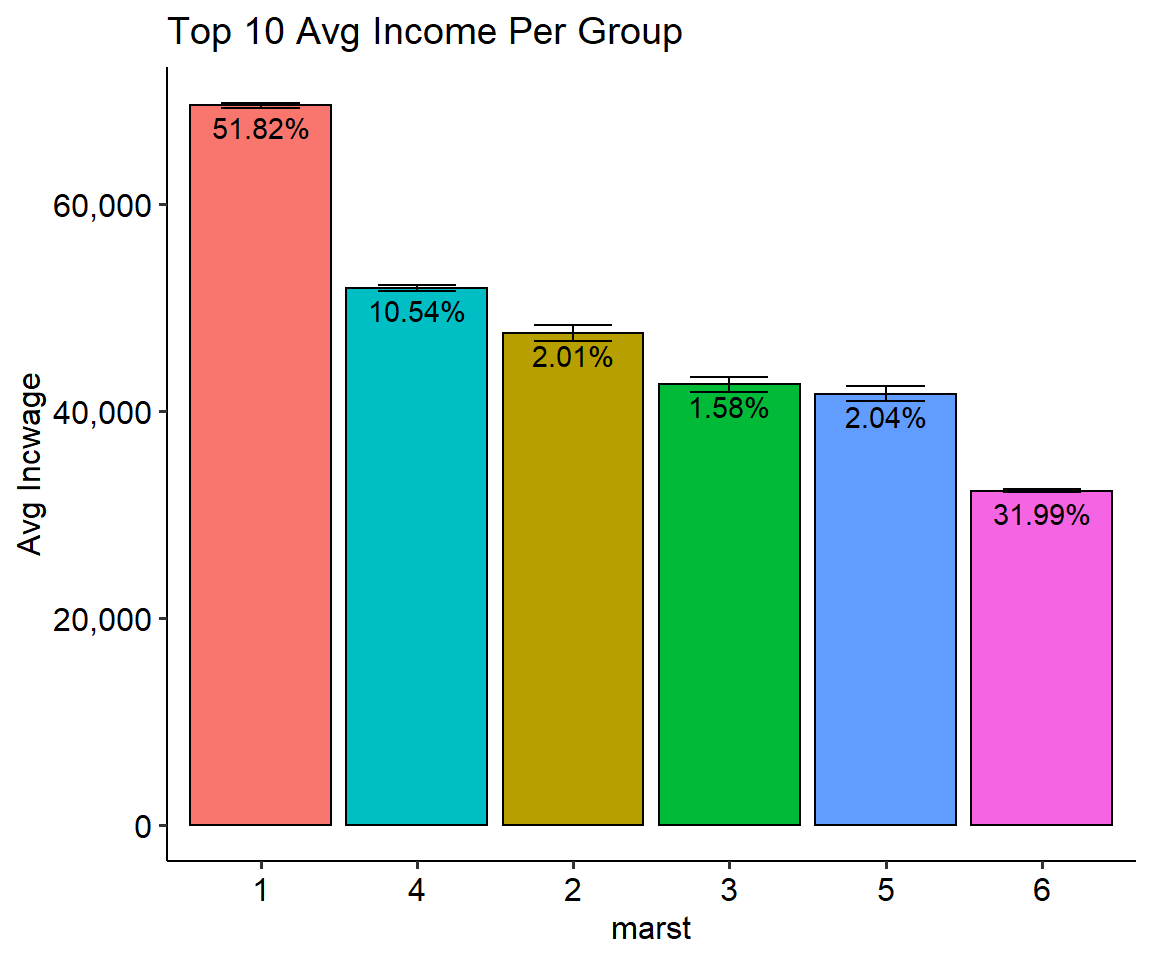
\includegraphics[width=0.9\linewidth]{imgs/preliminary_analysis/unnamed-chunk-7-4}
\end{figure}


\begin{figure}[ht]
	\centering
	\label{fig:unnamed-chunk-7-5}
	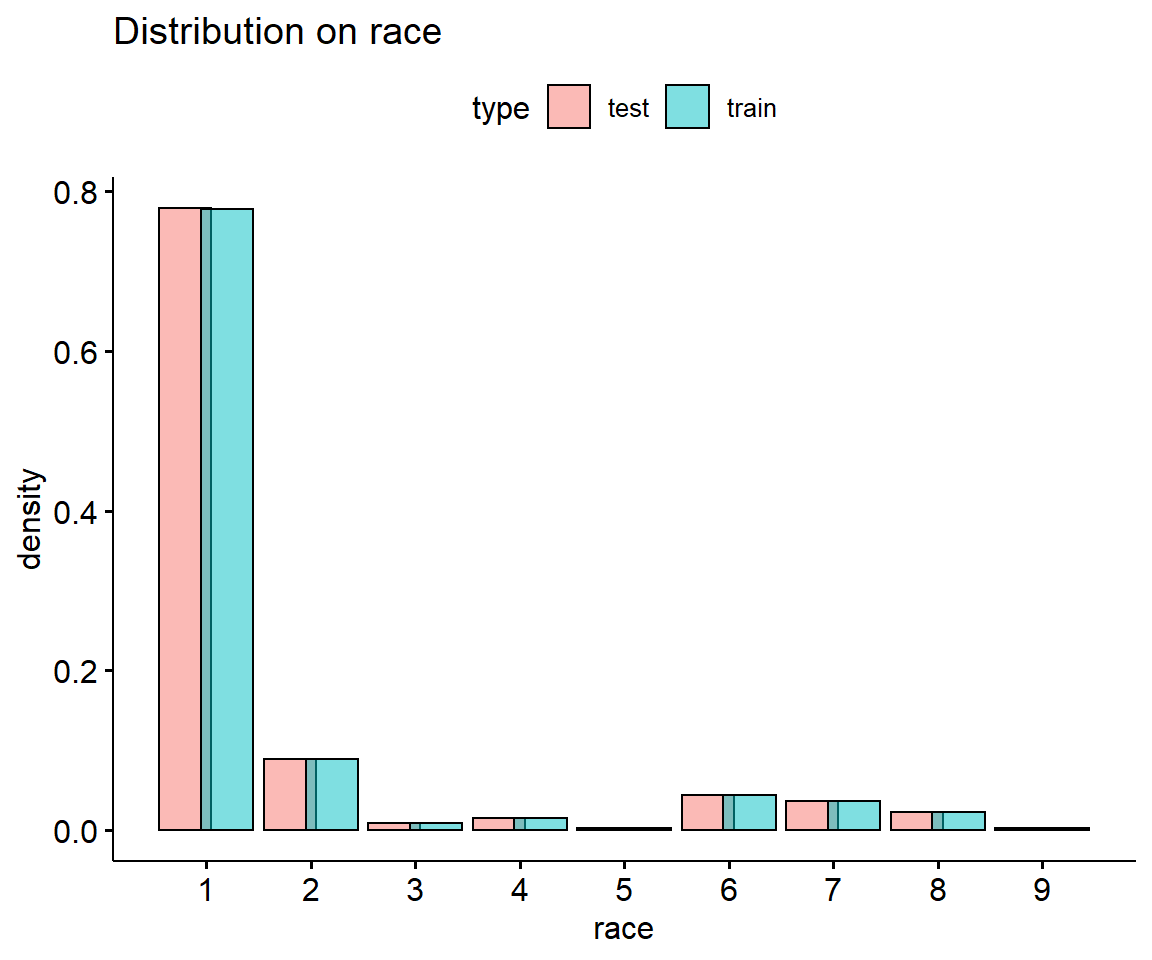
\includegraphics[width=0.9\linewidth]{imgs/preliminary_analysis/unnamed-chunk-7-5}
\end{figure}
\begin{figure}[ht]
	\centering

	\label{fig:unnamed-chunk-7-6}
	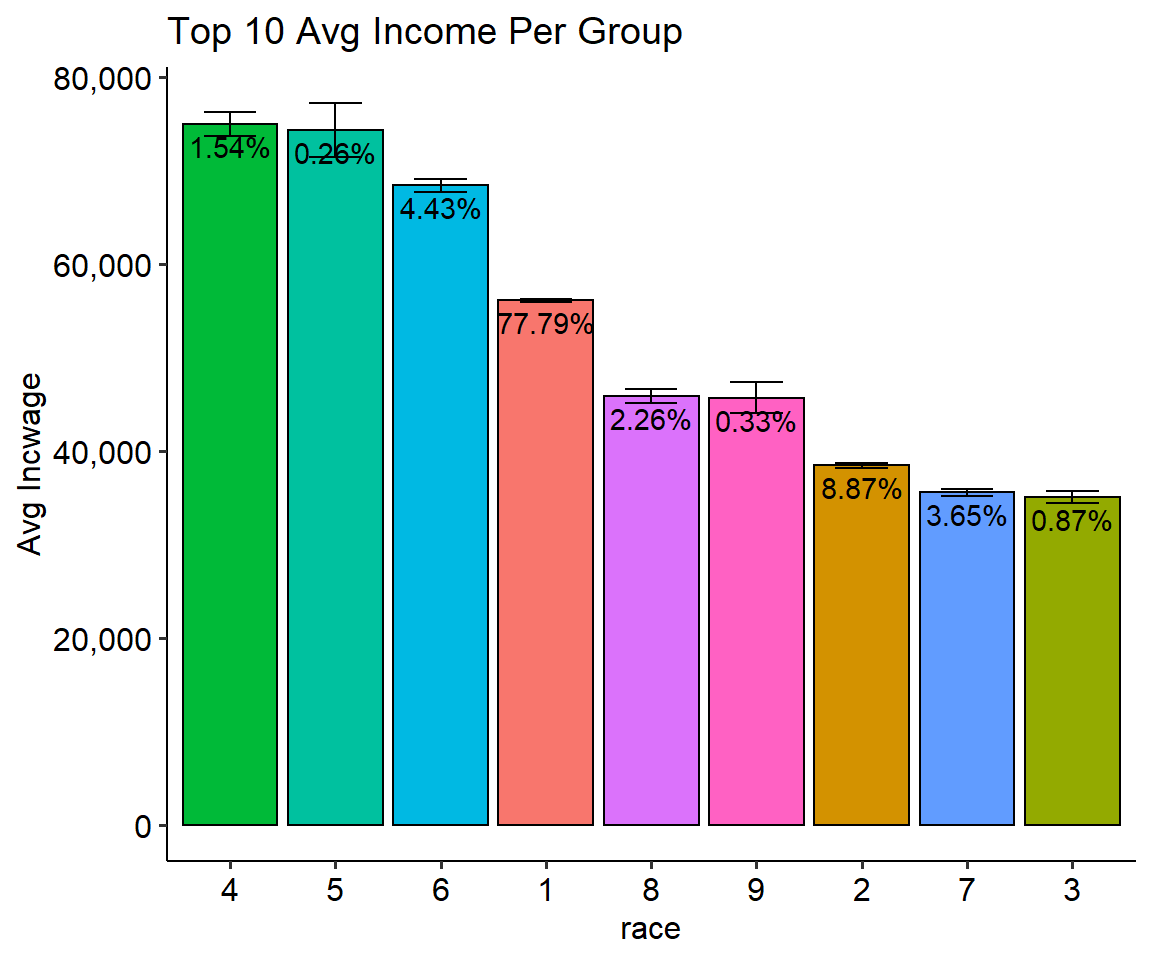
\includegraphics[width=0.9\linewidth]{imgs/preliminary_analysis/unnamed-chunk-7-6}
\end{figure}
\begin{figure}[ht]
	\centering
	\label{fig:unnamed-chunk-7-7}
	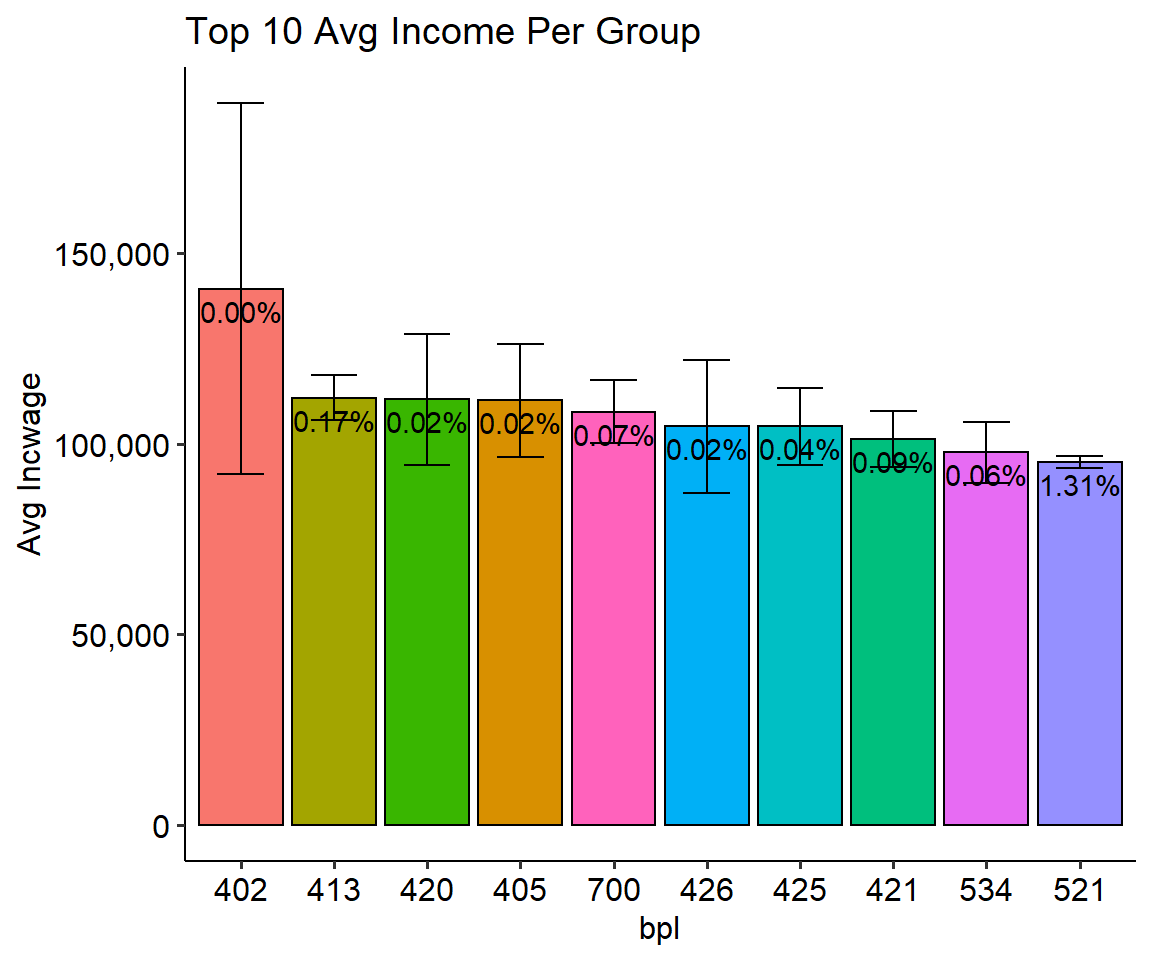
\includegraphics[width=0.9\linewidth]{imgs/preliminary_analysis/unnamed-chunk-7-7}
\end{figure}
\begin{figure}[ht]
	\centering

	\label{fig:unnamed-chunk-7-11}
	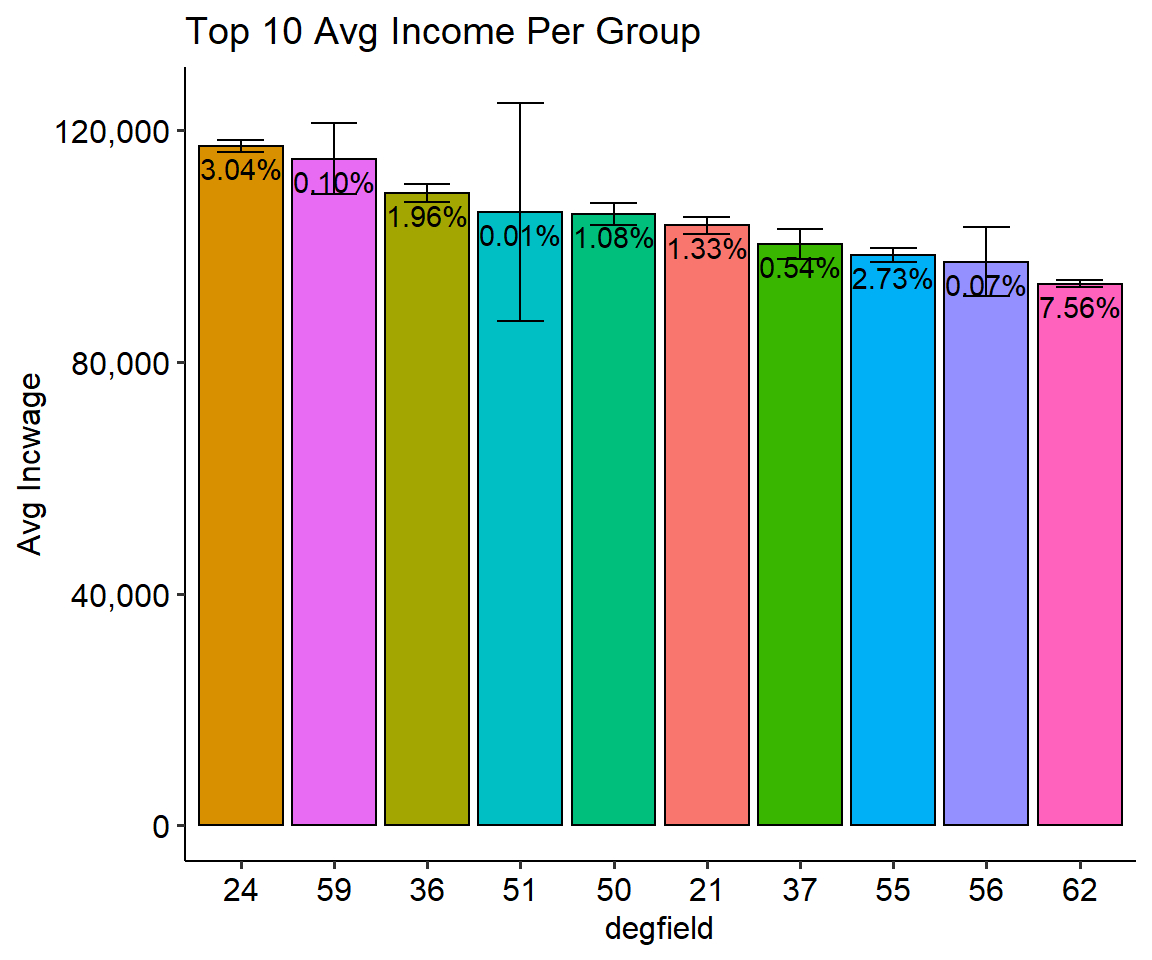
\includegraphics[width=0.9\linewidth]{imgs/preliminary_analysis/unnamed-chunk-7-11}
\end{figure}
\begin{figure}[ht]
	\centering

	\label{fig:unnamed-chunk-7-9}
	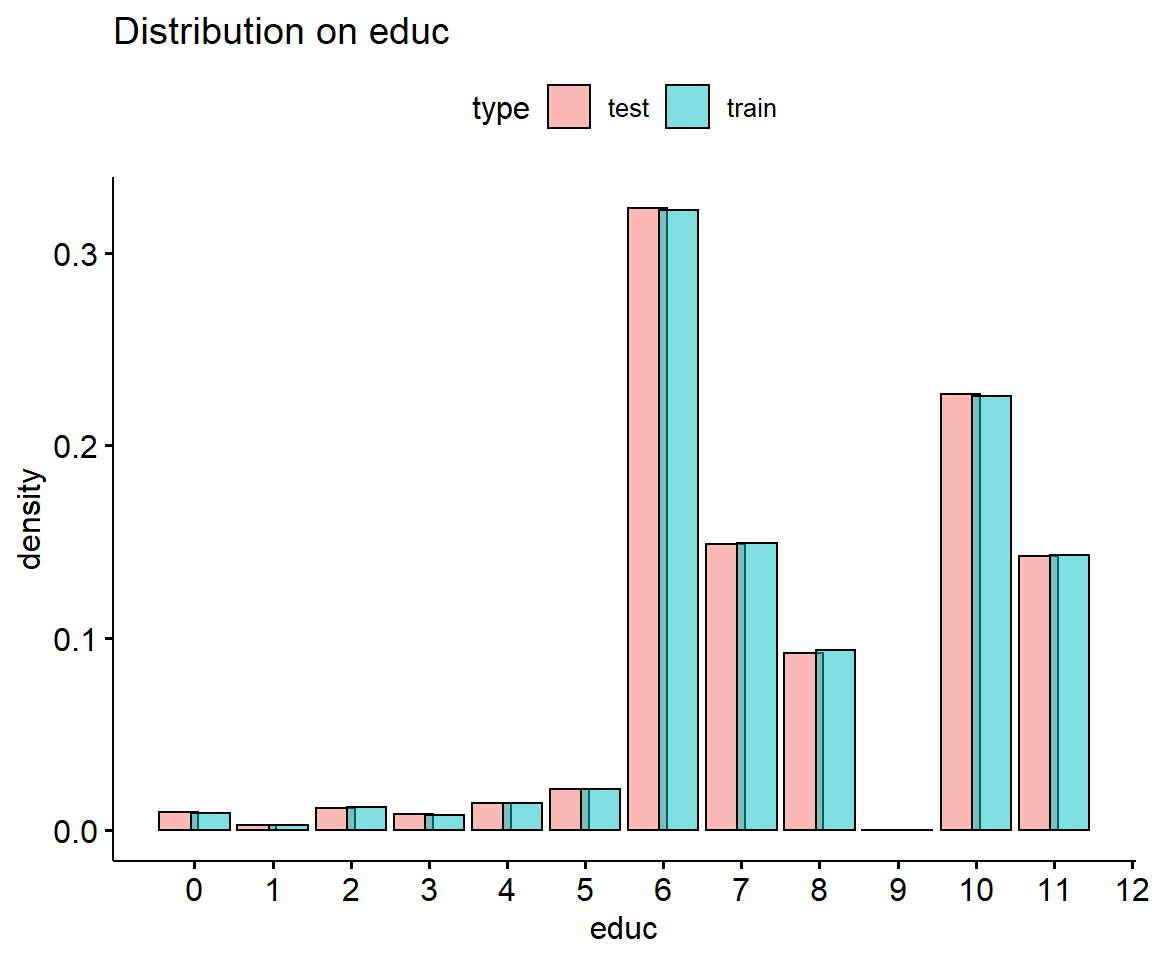
\includegraphics[width=0.9\linewidth]{imgs/preliminary_analysis/unnamed-chunk-7-9}
\end{figure}
 
\begin{figure}[ht]
	\centering
	\label{fig:unnamed-chunk-7-12}
	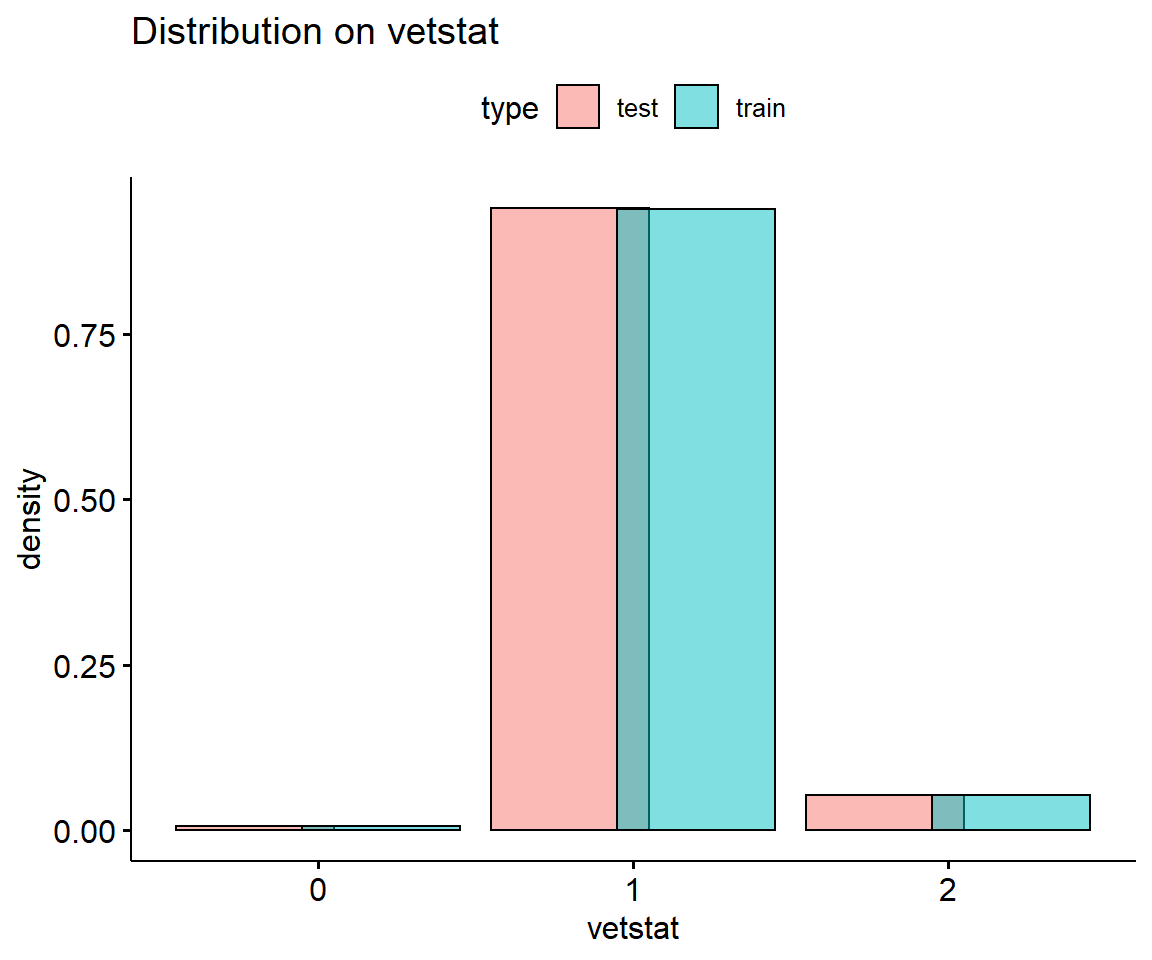
\includegraphics[width=0.9\linewidth]{imgs/preliminary_analysis/unnamed-chunk-7-12}
\end{figure}
\begin{figure}[ht]
	\centering
	\label{fig:unnamed-chunk-7-13}
	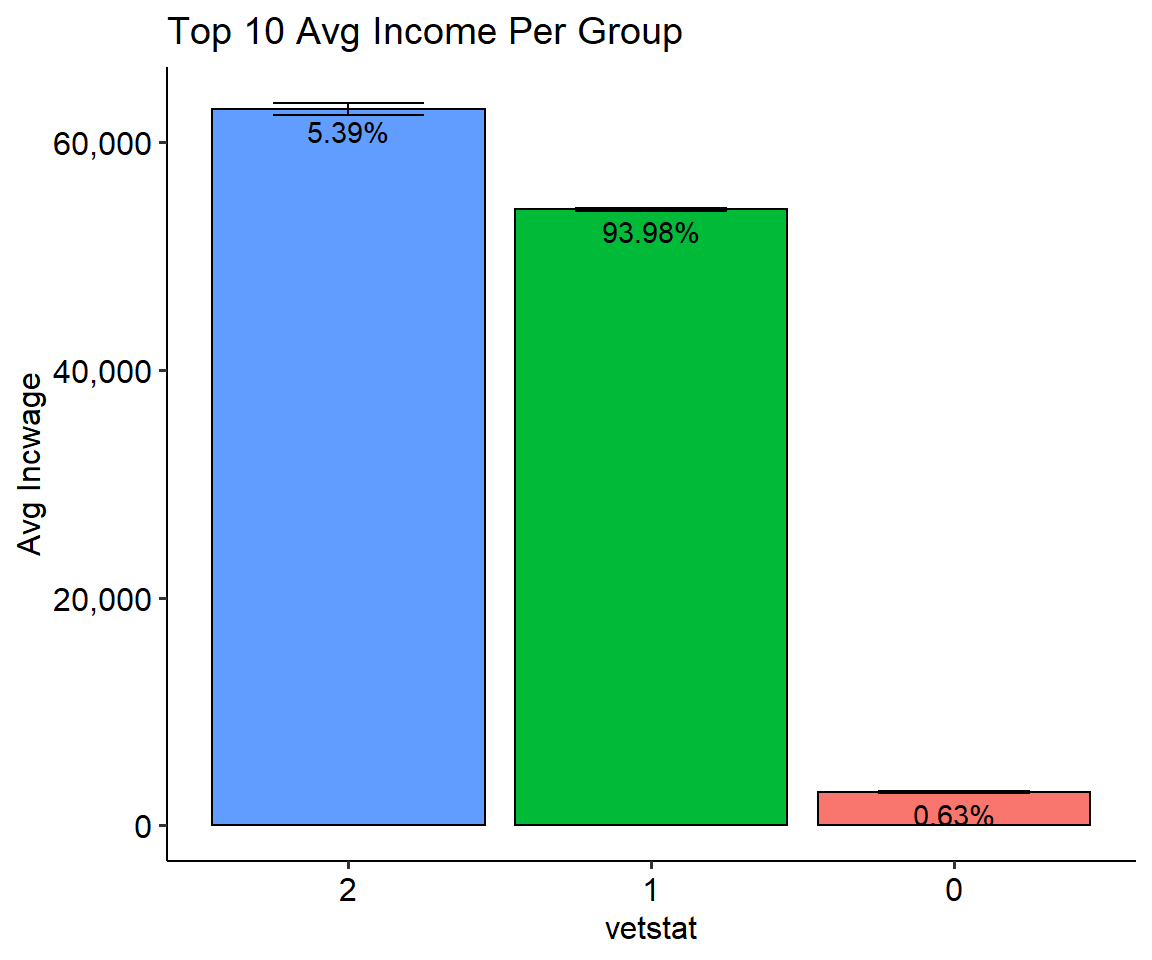
\includegraphics[width=0.9\linewidth]{imgs/preliminary_analysis/unnamed-chunk-7-13}
\end{figure}
\begin{figure}[ht]
	\centering
	\label{fig:unnamed-chunk-8-1}
	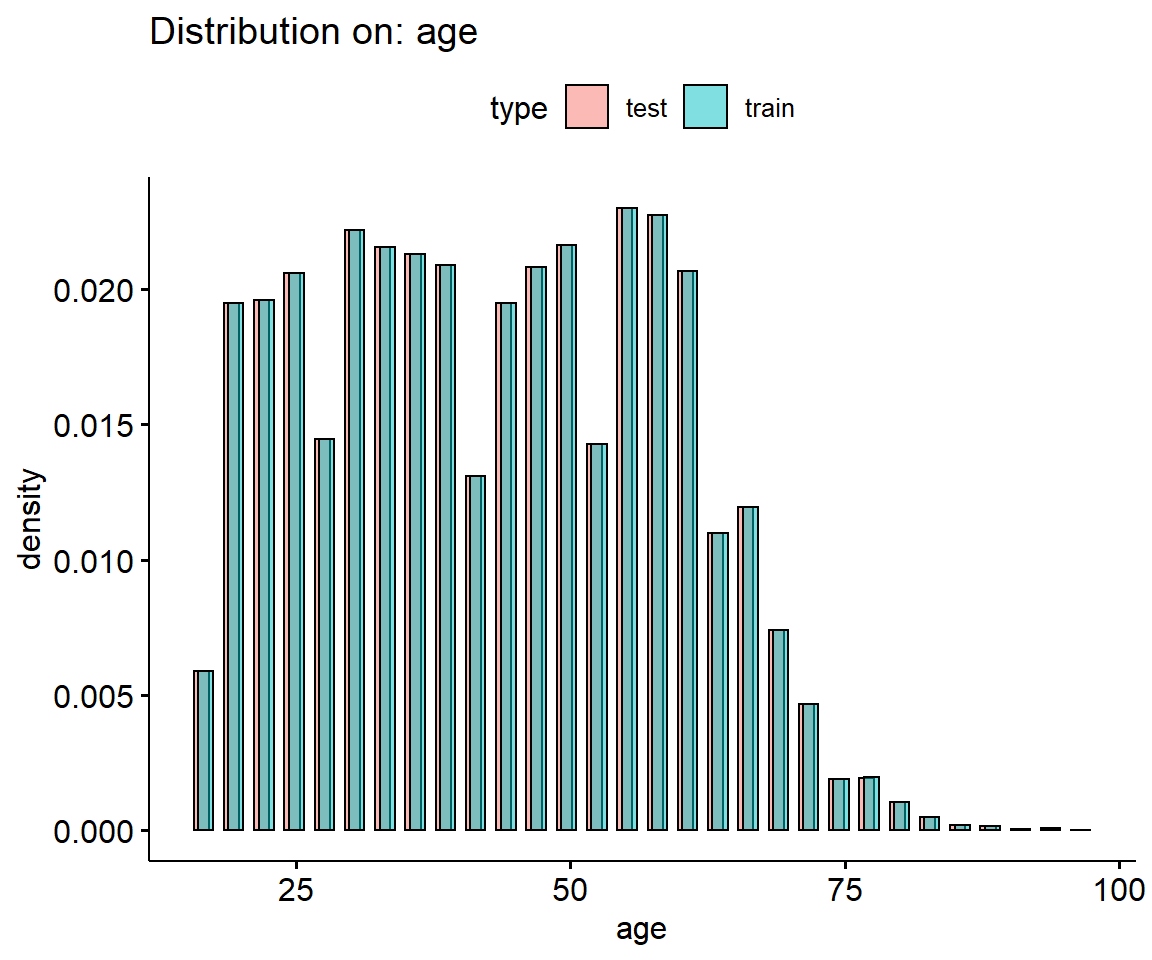
\includegraphics[width=0.9\linewidth]{imgs/preliminary_analysis/unnamed-chunk-8-1}
\end{figure}
\begin{figure}[ht]
	\centering

	\label{fig:unnamed-chunk-8-2}
	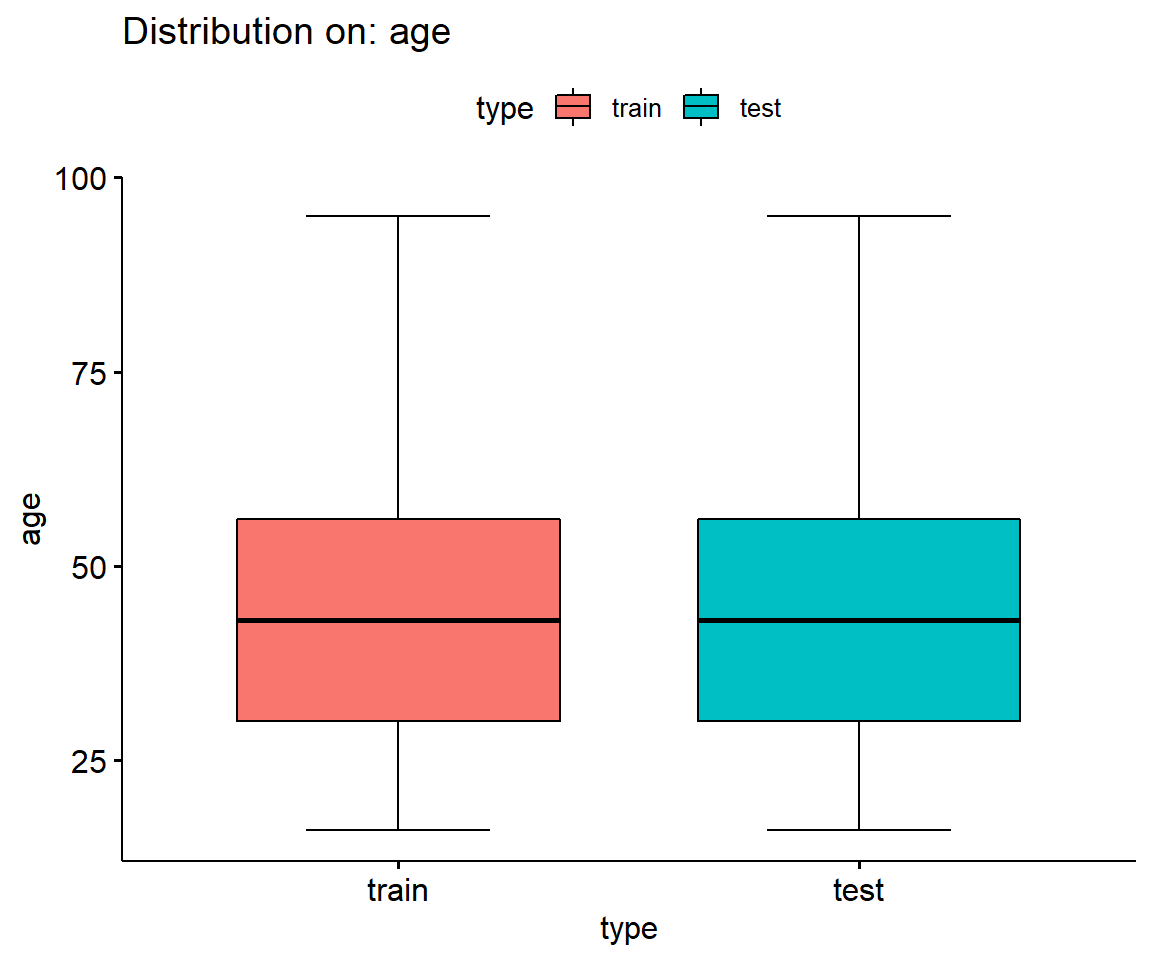
\includegraphics[width=0.9\linewidth]{imgs/preliminary_analysis/unnamed-chunk-8-2}
\end{figure}

\begin{figure}[ht]
	\centering

	\label{fig:unnamed-chunk-8-5}
	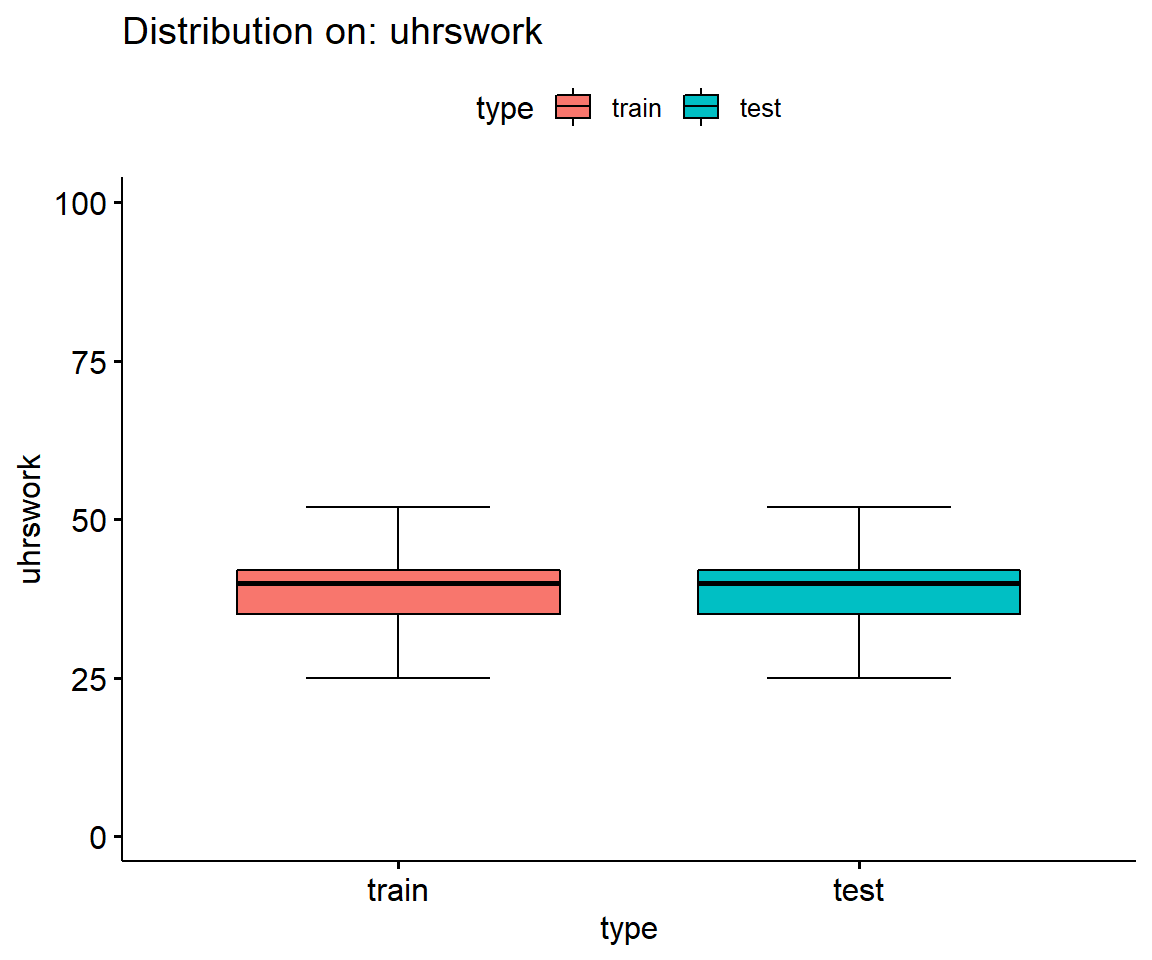
\includegraphics[width=0.9\linewidth]{imgs/preliminary_analysis/unnamed-chunk-8-5}
\end{figure}

\begin{figure}[ht]
	\centering
	\label{fig:unnamed-chunk-8-4}
	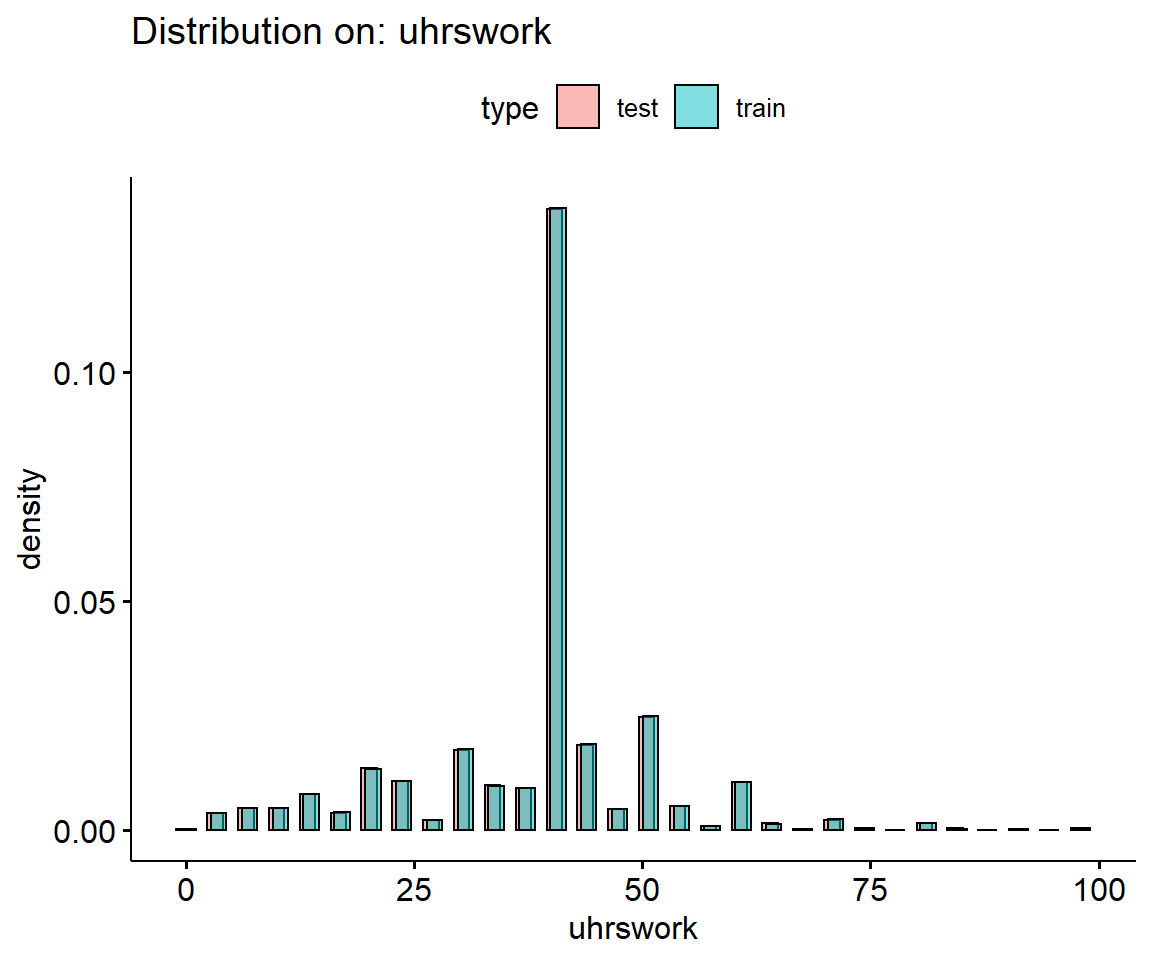
\includegraphics[width=0.9\linewidth]{imgs/preliminary_analysis/unnamed-chunk-8-4}
\end{figure}

\end{document}